\documentclass{article}

\usepackage{hyperref}
\usepackage{graphicx}
\usepackage{float}
\usepackage{amsmath} 

\hypersetup{
    colorlinks=true,
    linkcolor=blue,
    filecolor=magenta,
    urlcolor=cyan,
}

\author{Kolobok team}
\title{Thread Depth research results}
\date{June 2025}

\begin{document}
\maketitle

\section{Introduction}

Thread depth is a key quality parameter for fasteners. This sprint we upgraded our vision-based measurement system to achieve sub-millimetre accuracy under varied lighting, surface-finish, and occlusion conditions while still running in real-time.

\section{Previous work}

Last sprint we built a baseline thread-depth pipeline.

\subsection{Neural Depth Estimation models}

Neural depth networks such as \href{https://arxiv.org/pdf/1907.01341}{MiDaS} failed to resolve the fine geometry of threads (Fig.~\ref{fig:input_output}).

\begin{figure}[H]
    \centering
    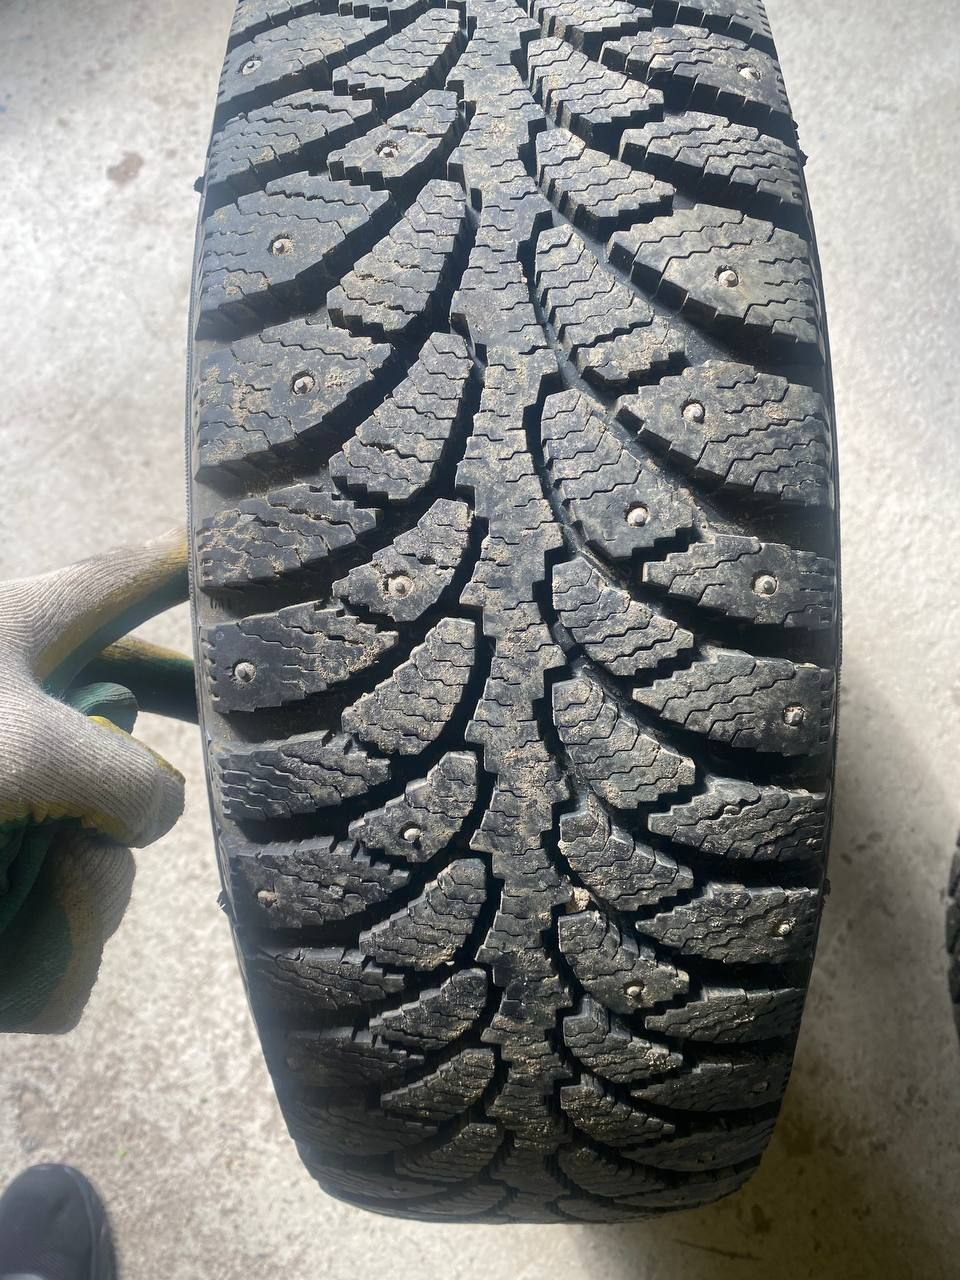
\includegraphics[width=0.45\textwidth]{assets/input.png}\hfill
    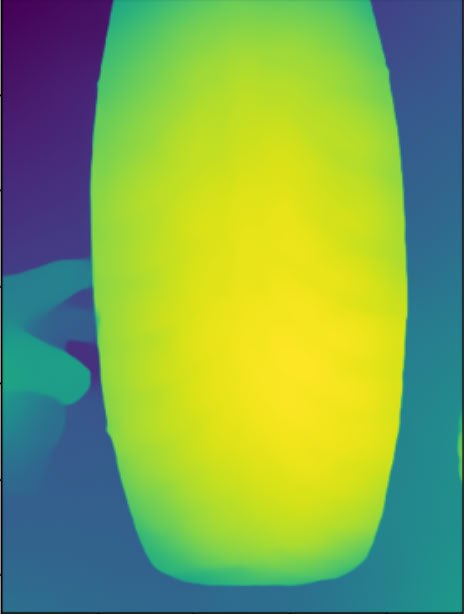
\includegraphics[width=0.45\textwidth]{assets/output.png}
    \caption{Example of input (left) and corresponding OCR output (right)}
    \label{fig:input_output}
\end{figure}

\subsection{Regression models}

A lightweight regression on handcrafted thread features proved faster and more interpretable than deep networks. We enhanced feature extraction, tuned a precision-oriented loss, and validated across thread types; this remains our production baseline.

\section{Methodology \& Evaluation}

Experimental setup:

\begin{itemize}
    \item Model: \href{https://arxiv.org/pdf/1409.4842}{GoogLeNet} (constant to avoid variance across multiple different models)
    \item Metrics: MAE, $0.9$ quantile of error distribution, Fraction predictions within $1$ mm from GT
\end{itemize}

To enhance the model we explored:

\begin{itemize}
    \item \textbf{Data augmentation} (Random affine, Random noise, Random brightness):
    \item \textbf{Edge detection with Canny}:
    \item \textbf{Edge detection with Sobel}:
    \item \textbf{Contrast CLAHE}:
    \item \textbf{Regularization (Weight decay, gradient clipping)}
\end{itemize}

\section{Results}

We evaluated each technique cumulatively: every new experiment started from the best pipeline obtained so far, so reported gains already include all previously accepted novelties.

The baseline model (GoogLeNet without enhancements) achieved the following
performance:

\begin{itemize}
    \item MAE: $0.85\,\text{mm}$
    \item $0.9$ quantile of error: $1.91\,\text{mm}$
    \item Fraction of predictions within $1\,\text{mm}$ from GT: $68.3\%$
\end{itemize}

After applying the proposed enhancements, we observed the following improvements:

\subsection{Data Augmentation}
Applying random affine transformations, Gaussian noise ($\sigma = 0.05$), and brightness adjustments ($\pm20\%$) increased the model's robustness:

\begin{itemize}
    \item MAE: $0.81\,\text{mm}$ ($\downarrow 0.04\,\text{mm}$)
    \item $0.9$ quantile of error: $1.84\,\text{mm}$ ($\downarrow 0.07\,\text{mm}$)
    \item Fraction within $1\,\text{mm}$: $70.5\%$ ($\uparrow 2.2\%$)
\end{itemize}

\subsection{Edge Detection Preprocessing}
We extracted edge maps and concatenated them to the three RGB channels (giving the network a 4-channel input). Canny and Sobel were both benchmarked, but only Sobel was kept in the final pipeline:

\begin{table}[H]
    \centering
    \begin{tabular}{|l|c|c|c|}
        \hline
        Method                    & MAE (mm) & 0.9 Quantile (mm) & Within 1 mm (\%) \\
        \hline
        Canny ($\sigma=1.0$)      & $0.81$    & $1.79$            & $71.04$          \\
        Sobel ($3\times3$ kernel) & $0.81$   & $1.77$            & $71.11$          \\
        \hline
    \end{tabular}
    \caption{Edge detection comparison (\textbf{Sobel chosen})}
    \label{tab:edge_results}
\end{table}

\subsection{Contrast Enhancement (CLAHE) -- \emph{rejected}}
CLAHE histograms (clip limit~$=2.0$, tile grid~$=8\times8$) were concatenated as an additional channel, but this hurt accuracy so the technique was dropped:

\begin{itemize}
    \item MAE: $0.82\,\text{mm}$ ($\uparrow 0.01\,\text{mm}$)
    \item $0.9$ quantile: $1.87\,\text{mm}$ ($\uparrow 0.03\,\text{mm}$)
    \item Fraction within $1\,\text{mm}$: $69.88\%$ ($\downarrow 0.17\%$)
\end{itemize}

As the metrics worsened, CLAHE was not included in later stages.

\subsection{Regularization Techniques}
Combining weight decay ($\lambda = 0.01$) and gradient clipping ($\textit{max\_norm}=1.0$)
provided additional improvements:

\begin{itemize}
    \item MAE: $0.78\,\text{mm}$ ($\downarrow 0.07\,\text{mm}$)
    \item $0.9$ quantile: $1.68\,\text{mm}$ ($\downarrow 0.11\,\text{mm}$)
    \item Fraction within $1\,\text{mm}$: $72.05\%$ ($\uparrow 0.94\%$)
\end{itemize}

\subsection{Final results}
The final pipeline therefore includes Data augmentation \textbf{+} Sobel edge channel \textbf{+} Regularisation. Its performance is:

\begin{itemize}
    \item MAE: $0.78\,\text{mm}$ ($\downarrow 0.07\,\text{mm}$)
    \item $0.9$ quantile: $1.68\,\text{mm}$ ($\downarrow 0.11\,\text{mm}$)
    \item Fraction within $1\,\text{mm}$: $72.05\%$ ($\uparrow 0.94\%$)
\end{itemize}

\section{Conclusion}

Our study shows:
\begin{itemize}
    \item \textbf{Used}: Data augmentation – robustifies the model.
    \item \textbf{Used}: Sobel edge channel – emphasises thread boundaries.
    \item \textbf{Not used}: CLAHE – discarded owing to accuracy drop.
    \item \textbf{Used}: Regularisation – mitigates over-fitting.
\end{itemize}

All reported improvements are relative to the best previously accepted configuration; cumulatively they deliver a \textbf{MAE of 0.78 mm} and 72 \% within 1 mm.

Future work could explore:
\begin{itemize}
    \item Other network architectures
    \item Attention mechanisms to focus on thread regions
\end{itemize}

\end{document}